\documentclass[review]{siamart0516}

\usepackage{microtype}

\usepackage{newunicodechar}
\newunicodechar{α}{\ensuremath \alpha}
\newunicodechar{β}{\ensuremath \beta}

\usepackage{amsmath}
\DeclareMathOperator{\E}{E}
\DeclareMathOperator{\Var}{Var}

\usepackage{listings}
\lstdefinelanguage{julia}{
  basicstyle=\small\ttfamily,
  showspaces=false,
  showstringspaces=false,
  keywordstyle={\textbf},
  morekeywords={if,else,elseif,while,for,begin,end,quote,try,catch,return,local,abstract,function,generated,macro,ccall,finally,typealias,break,continue,type,global,module,using,import,export,const,let,bitstype,do,in,baremodule,importall,immutable},
  escapeinside={~}{~},
  morecomment=[l]{\#},
  commentstyle={},
  morestring=[b]",
}
\lstset{language=julia, numbers=left, numberstyle=\tiny, mathescape=true}

\usepackage{algorithm}
\usepackage{algorithmic}
\bibliographystyle{siamplain}

\usepackage{pgfplots}
\usepackage{subcaption}

\usepackage{pifont}
\newcommand{\cmark}{\ding{51}}%
\newcommand{\xmark}{\ding{55}}%

\title{Fast computation of the principal components of genomics data in Julia
    \thanks{This
        work was supported by the Intel Science and Technology Center for Big Data.
	}}

\author{%
    Jiahao Chen
    \thanks{Computer Science and Artificial Intelligence Laboratory,
           Massachusetts Institute of Technology,
           Cambridge, Massachusetts, 02139 ({\tt jiahao@mit.edu})}
    %
    \and
    Andreas Noack
    \thanks{Computer Science and Artificial Intelligence Laboratory,
            Massachusetts Institute of Technology,
            Cambridge, Massachusetts, 02139 ({\tt noack@mit.edu})}
    \and
    Alan Edelman
    \thanks{Department of Mathematics and Computer Science and Artificial Intelligence Laboratory,
            Massachusetts Institute of Technology,
            Cambridge, Massachusetts, 02139 ({\tt edelman@mit.edu})}
}


\begin{document}

\maketitle

\tableofcontents

\begin{abstract}
Finding the largest few principal components of a matrix of genetic data is a
common task in genome-wide association studies (GWASs), both for dimensionality
reduction and for identifying unwanted factors of variation.
We describe a simple random matrix model for matrices that arise in GWASs,
showing that the singular values have a bulk behavior that obeys a
Marchenko-Pastur distributed with a handful of large outliers.
We also implement Golub-Kahan-Lanczos (GKL) bidiagonalization in the Julia
programming language, providing thick restarting and a choice between full
and partial reorthongalization strategies to control numerical roundoff.
Our implementation of GKL bidiagonalization is up to 36 times faster than
software tools used commonly in genomics data analysis for computing principal
components, such as EIGENSOFT and FlashPCA, which use dense LAPACK routines
and randomized subspace iteration respectively.
\end{abstract}

\begin{keywords}
    singular value decomposition,
    principal components analysis,
    genome-wide association studies,
    statistical genetics,
    Lanczos bidiagonalization,
    Julia programming language,
    subspace iteration
\end{keywords}

\begin{AMS}
    65F15, 97N80
\end{AMS}

\pagestyle{myheadings}
\thispagestyle{plain}
\markboth{J. CHEN, A. NOACK AND A. EDELMAN}{Principal components of genomics data in Julia}

\section{Principal components of genomics data}

Personalized medicine or precision medicine is a growing movement to tailor treatments of disease
to an individual's sensitivities to treatment, allergies, or other genetic
predispositions, using all available data about an individual~\cite{Desmond2012}.
Developers of personalized medical treatments are therefore interested in how an
individual's genome, both in isolation and within the context of the wider human
population, can be used to predict desired clinical outcomes (known as
comorbidities or phenotypes)~\cite[Ch. 8]{Laird2011}.
Genome-wide association studies (GWASs) are a new and popular technique for
studying the significance of human genome data, by studying the associate genotype
variation with phenotype variations in outcome variables e.g.\ the clinical
observation of a disease.

The genome data used in
GWASs are are often encoded in a matrix expressing the number of mutations
from a reference genome, which we will refer to as a \textit{genomics matrix}.
By convention, the genomics matrix is indexed by patients (or other test
subjects) on the rows and gene markers on the columns which represent some
coordinate or locus within the human genome. A common example of gene markers are
single nucleotide polymorphisms (SNPs), which represent gene positions with
pointwise mutations of interest that express variation in the genotype across
humans. Oftentimes, the explanatory data in a GWAS are simply called SNP data.
Since most human cells are at most diploid, i.e.\ have two sets of chromosomes,
the matrix elements can only be 0, 1, or 2 (or missing).

There are two major confounding sources of variation which are considered in
the analysis of human genome data, each of which have significance for the
spectral properties of the matrix:

\paragraph{Population stratification/admixing}
Population stratification is the phenomenon of common genetic variation within
mutually exclusive subpopulations defined along racial, ethnic or geographic
divisions~\cite{Pritchard1999,Cardon2003}. (Admixture models relax the mutual
exclusion constraint~\cite{Devlin1999,Sankararaman2008}.)
In linear algebraic terms, the genomics matrix will have a low rank component
with large singular values.

\paragraph{Cryptic relatedness}
Sometimes called kinship or inbreeding, cryptic relatedness is an increase in
sampling bias in the columns (human genomes) produced by having common ancestors,
thus increasing the nominally observed frequency of certain
mutations~\cite{Voight2005,Astle2009}. Relatedness is usually detected and removed in
a separate preprocessing step, but it is not always possible to remove
fully~\cite{PLINK}. Any remaining related samples will
result in (near) linear dependencies in the rows of the genomic matrix,
leading to the presence of several singular values that are very small or zero.

Principal component analysis (PCA) was historically first used as a dimensionality
reduction technique to summarize the variation in the human genes and study its
implications for human evolution in relation to other factors such as
geography and history~\cite{Menozzi1978,Cavalli1994,Novembre2008}.
However, we will focus on the more modern use of principal components (PCs) to
represent the confounding effects of population substructure in the statistical
modeling of GWASs~\cite{Chen2003,Patterson2006,Price2006,Zhu2002,Zhang2003}.

Genomics matrices form an interesting use case for the classical techniques of
numerical linear algebra, as the amount of sequenced genome data grows
exponentially~\cite{Stephens2015}. As the price of sequencing genome data declines
rapidly, genomics studies involving hundreds of thousands of individuals (columns)
are already commonplace today, with order of magnitude growth expected within the next year or two. Therefore, genomics researchers will require access to the best
available algorithms for parallel computing and numerical linear algebra to
handle the increasing demands of data processing and dimensionality reduction.


\subsection{The statistical significance of principal components}

The main statistical tool used in GWAS is regression, using some model that
associates genotype variation with phenotype variation.
While correlation does not imply causation in and of itself, the central dogma
of molecular biology states that causality flows from genetic data in DNA and RNA
to phenotype data in expressed proteins~\cite{Crick1970}. Consequently, correlations between genotypes and phenotypes could in theory have causal significance.
The \emph{linear} regression model is one the simplest useful models, and can be
motivated in several different ways. One way is in terms of least squares
minimization to find the coefficients that minimize the sum of squared distances
between a hyperplane and the observations. Another way to formulate the problem
as finding a projection of the a vector of observations down onto the space
spanned by the vectors of explanatory variables.
One caveat in statistical studies is the assumption that the observations are
randomly sampled with replacement, and hence that the observations can be
assumed to be independent. In the context of statistical genomics, the
independence assumption is one of several bundled into the principle of
Hardy-Weinberg equilibrium~\cite{Hardy1908,Weinberg1908}, which is commonly
assumed in statistical genetics~\cite{Laird2011}. However, caution must be taken
to remove possible sampling bias due to the collection of genetic data from
patients from a single hospital or hospital network, on top of sampling bias
introduced by not treating the presence of population substructure.


\subsection{The linear regression model}

The statistical theory of regressing phenotypes against genotypes is best expressed
in terms from conditional expectations. If we for individual $i$ denote the genotype measurement by $x_i$ and the phenotype measurement by $y_i$, the conditional
expectation of interest can be written as $\E(y_i|x_i)=\beta_0 + \beta_1 x_i$.
A popular formulation of the this model is
%
\begin{equation*}
    y_i = \beta_0 + x_i \beta_1 + \varepsilon_i\quad i=1,\dots,n
\end{equation*}
%
where $n$ is the number of observations which in this case would be the number of individuals for which we have genotype data.
The variable $\varepsilon_i$ is called the error term and must satisfy $\E(\varepsilon_i|x_i)=0$.
More generally, $\varepsilon_i$ is the conditional distribution $y_i - \beta_0 - x_i\beta_1|x_i$.

The multivariate expression can be written conveniently in matrix form

\begin{equation}
\label{eq:linreg}
    y = X\beta + \varepsilon
\end{equation}
%
with
%
\begin{equation*}
    X = \begin{pmatrix}
        1 & x_1\\
        \vdots & \vdots \\
        1 & x_n
    \end{pmatrix}
\end{equation*}
%
and in this notation, the well-known least squares estimator for the coefficient
$\beta$ can be written as
%
\begin{equation}
\label{eq:ols}
    \hat{\beta} = (X^TX)^{-1}X^Ty.
\end{equation}

The conditional probability treatment demonstrates that when $(x_i,y_i)$ pairs
are considered to be random variables, then $\hat{\beta}$ is also a random
variable, with its mean and variance quantifying uncertainty about the least
squares solution.
First, notice that the least squares estimator \eqref{eq:ols} can be written
%
\begin{equation*}
    \hat{\beta} = \beta + (X^TX)^{-1}X^T\varepsilon
\end{equation*}
%
and the expected value of the estimator is
%
\begin{equation}
    \E(\hat{\beta}|X) = \E(\beta + (X^TX)^{-1}X^T\varepsilon|X) =
        \beta + (X^TX)^{-1}X^T\E(\varepsilon|X) = \beta
\end{equation}
%
which means that the estimator is \emph{unbiased}. Statisticians are interested in the variability of $\hat{\beta}$ under changes to the data that could be considered small errors. The most common measurement for the variability of an estimator is the (conditional) variance, i.e.
%
\begin{equation*}
    \Var(\hat{\beta}|X) = \Var(\beta + (X^TX)^{-1}X^T\varepsilon|X) =
        (X^TX)^{-1}X^T\Var(\varepsilon|X)X(X^TX)^{-1}.
\end{equation*}

This shows that variance of $\hat{\beta}$ depends on the (conditional) variance of $\varepsilon$, which has not been discussed yet. In classical treatments of the linear regression model it is typically assumed that, conditionally on $x_i$, the $y_i$s are independent and the have the same variance which is the same as $\Var(\varepsilon|X)=\sigma^2 I$ for some unknown scalar $\sigma^2$. Under this assumption, the variance of $\hat{\beta}$ reduces to $\sigma^2 (X^TX)^{-1}$. The magnitude of this quantity is unknown because $\sigma^2$ is an unknown parameter but $\sigma^2$ can be \emph{estimated} from the data. The usual estimator is
$\hat{\sigma}^2=\frac{1}{n} \|\hat{\varepsilon}\|^2$
where $\hat{\varepsilon} = y - X\hat{\beta}$.
This leads to the estimate of the (conditional) variance of the estimator $\widehat{\Var(\hat{\beta}|X)} = \hat{\sigma}^2(X^TX)^{-1}$.

The independence assumption is often used in statistics and can be justified from an assumption of random sampling with replacement. In studies where data is passively collected, this might not be a reasonable assumption as explained in the previous section. Non-random sampling might lead to correlation between the phenotypes even after conditioning on the genotypes. In consequence of that, $\Var(\varepsilon|X)$ will no longer be diagonal, but have some general positive definite structure $\Sigma$ and $\Var(\hat{\beta}|X)=(X^TX)^{-1}X^T\Sigma X(X^TX)^{-1}$. Since $\Sigma$ in general consists of $\frac{n(n+1)}{2}$ parameters, it cannot be estimated consistently.

In order to analyze the problem with correlated observations, it is convenient to decompose the error into a part that contains the cross-individual correlation and a part that is diagonal and therefore only describes the variance for each individual. This may be written as
%
\begin{equation*}
    y_i = \beta_0 + x_i\beta_1 + \eta_i + \xi_i
\end{equation*}
%
where is assumed that $\Var(\eta|X)=\Sigma_\eta$ and $\Var(\xi|X)=\sigma^2_\xi I$. Furthermore, it is assumes that the two error terms are independent.


\label{sec:regress-correction}
\subsubsection{Fixed effect estimation}

One way to produce a reliable estimate of the variance of $\hat{\beta}$ is to come up with a set of variables $z_1,\dots,z_k$ that proxies the correlation between the observations, i.e.\ $\eta=Z\gamma$. By simply including the variables $z_1,\dots,z_k$ in the regression model, it possible to remove the correlation which distorts the variance estimate for $\hat{\beta}$. For the regression $y|X,Z$, we get the least squares estimator
\begin{equation*}
    \begin{pmatrix}\hat{\beta} \\ \hat{\gamma}\end{pmatrix} =
    \begin{pmatrix}
        X^TX & X^TZ \\ Z^TX & Z^TZ
    \end{pmatrix}^{-1}\!\!
    \begin{pmatrix}
        X^T \\ Z^T
    \end{pmatrix}
    (X\beta + Z\gamma + \xi)=
    \theta +
            \begin{pmatrix}
        X^TX & X^TZ \\ Z^TX & Z^TZ
    \end{pmatrix}^{-1}\!\!
    \begin{pmatrix}
        X^T \\ Z^T
    \end{pmatrix}\xi,
\end{equation*}
which has variance
\begin{equation*}
    \Var\left(\begin{pmatrix}\hat{\beta} \\ \hat{\gamma}\end{pmatrix}|X,Z\right)=\sigma_\xi^2
        \begin{pmatrix} X^TX & X^TZ \\ Z^TX & Z^TZ \end{pmatrix}^{-1}.
\end{equation*}

In many applications, a few pricipal components of the covariance matrix of the complete SNP dataset is used as a proxy for the correlation between individuals. Computing principal components is therefore often a first step in analyzing GWASs.


\subsection{Software for computing the principal components of genomics data}

The software stack for GWAS is generally based on command line tools written completely in C/C++. Not only is the core computational algorithm written in C/C++ but also much of the pre- and postprocessing of the data. The datasets can be large but and the computations at times heavy but it has been a surprise to learn the extend to which analyses are carried out directly from the command line instead of using higher level languages like Matlab, R, or Python. This choice seems to limit the tools available to the analysts because, unless he is a C/C++ programmer, the programmer is restricted to the set of options included in the command line tool.

Two major packages exist for computing the PCA in the GWAS software stack. The package \emph{EIGENSOFT} accompanied~\cite{Patterson2006} which popularized the use of PCA in GWAS. In the original version of the package, the routine \texttt{smartpca} for computing the PCA of a SNP matrix was based on an eigenvalue solver from LAPACK. In consequence, all the eigenvalues and vectors of the SNP matrix were computed even though only a few of them were used as principal components. Computing the full decomposition is inefficient and as the number of available samples has grown over the year, this approach has become impractical.

More recently, \emph{FlashPCA}~\cite{abraham2014fast}, has emerged as a potentially faster alternative to EIGENSOFT's \texttt{smartpca}. The PCA routine is based on a truncated SVD algorithm described in~\cite{halko2011finding}. More specifically, FlashPCA uses a subspace iteration scheme with either columnwise scaling (FlashPCA 1) or orthogonalization by QR (FlashPCA 2) in each iteration. The convergence criterion is based on the average of squared elementwise distance between the the bases for iteration $i-1$ and $i$. The QR orthogonalization step in the implementation of FlashPCA routine deviates from the algorithm in described~\cite{abraham2014fast} which only normalizes columnwise. Our conjecture was that this change was made to avoid loss of orthogonality in the subspace basis and the author of the package has confirmed this. In consequence, the timings in~\cite{abraham2014fast} do not correspond to the performance of the software run with default settings since the QR orthogonalization is much slower than the columnwise normalization. Furthermore, a degenerate basis might also converge much faster because it eventually converges to the single largest eigenvalue.

For people trained in numerical methods, it is surprising that well established packages such as ARPACK and PROPACK are not used much in genomics. In particular since both ARPACK and PROPACK have convenient wrapper libraries in both R, Python, and MATLAB. This might be explained by the pronounced use of C/C++, where calling ARPACK and PROPACK are relatively more demanding, combined with the fact that iterative methods are traditionally not part of the curriculum in biology, medicine, or statistics.

\begin{table}
    \centering
    \caption{Software comparison}
    \begin{tabular}{ccc}
        Software  & Algorithm                              & Used in genomics \\
        EIGENSOFT & Householder bidiagonalization (LAPACK) & \cmark \\
        FlashPCA  & Block power                            & \cmark \\
        ARPACK    & Lanczos, $X^TX$                        & \xmark \\
        PROPACK   & Lanczos                                & \xmark
    \end{tabular}
\end{table}

\label{sec:model}
\section{A simple model for genomics data}

In this section we present a very simple random model which accurately mimics
the spectral features observed in real data matrices.
We hypothesize that the spectral properties of human patient genotype data can
be modeled the Julia code in Algorithm~\ref{code:model}, which captures the
confounding effects of population stratification and kinship.
The former is modeled by setting randomly select subblocks to the same value,
whereas the latter is modeled by duplicating rows, thus purposely introducing
linear dependence into the column space. This model, while simplistic, can be
tuned to reproduce the scree plot observed in empirical data matrices and we
expect that such models may be of interest to researchers developing numerical
algorithms that lack access to actual data, which are often access-restricted
due to clinical privacy.

\begin{algorithm}
\caption{A simple model for human genotype data matrices in Julia
\label{code:model}}
\begin{lstlisting}
"""
Inputs:
- m: number of rows (gene markers)
- n: number of columns (patients)
- r: number of subblocks to model population admixing
- nsignal: number of entries to represent signal
- rkins: fraction of columns to duplicate

Output:
- A: a dense matrix of size m x n with matrix elements 0, 1 or 2
"""
function model(m, n, r, nsignal, rkins)
    A = zeros(m, n)
    #Model population admixing
    #by randomly setting a subblock to the same value, k
    for i=1:r
        k = rand(0:2)
        r1 = randrange(m)
        r2 = randrange(n)
        A[r1, r2] = k
    end

    #Model signal
    for i=1:nsignal
        A[rand(1:m), rand(1:n)] = rand(0:2)
    end

    #Model kinship by duplicating rows
    nkins = round(Int, rkins*m)
    for i=1:nkins
        A[rand(1:m), :] = A[rand(1:m), :]
    end
    return A
end

function randrange(n)
    i1 = rand(1:n)
    i2 = rand(1:n)
    if i1 > i2
        return i2:i1
    else
        return i1:i2
    end
end
\end{lstlisting}
\end{algorithm}

Algorithm~\ref{code:model} describes a \verb|model| function, which creates a
dense, synthetic data matrix of size $m\times n$. The synthetic data is
generated in three steps. First, randomly select $r$ rectangular submatrices
(which may overlap) and set the elements of each submatrix to the same value.
This process simulates crudely the effects of population admixture, where
each subpopulation has a common block of mutations that vary together, and the
possibility of overlap resembles the effect of mixing different subpopulations
together. (This step uses the auxiliary \verb|randrange| function, which returns
a valid Julia range that is a subinterval of the range \verb|1:n|.)
Second, model the genotype of interest by randomly setting $nsignal$ matrix
element randomly to 0, 1 or 2.
Third, simulate the effects of kinship by choosing a fraction $rkins$ of the
rows to duplicate.

The model is clearly a very crude approximation to genotype data with the
confounding effects of population substructure. There is little overt control
over the admixture process, the precise distribution over matrix elements, and
all related patients are assumed to have identical genotypes. Nevertheless, the
model generates realistic distributions of singular values which mimic closely
what we have observed in that of real world genomics matrices.
Figure~\ref{fig:empirical-spectrum} shows the distribution of singular values
generated by our model with parameters $m=81700$, $n=41505$, $r=10$,
$nsignal=mn$, $rkins=0.017$.
There are a handful of ($\approx r$) large singular values,
while the rest follow a bulk distribution from random matrix theory known as the
Marchenko-Pastur law~\cite{Marchenko1967} with parameter $\rho = 1.86$.


\begin{figure}

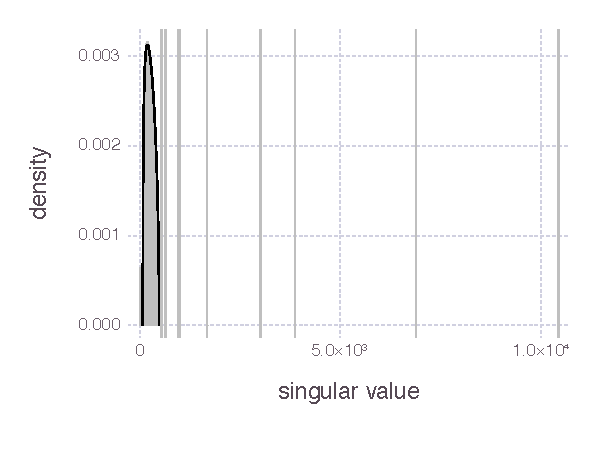
\includegraphics[width=0.45\textwidth]{fig/synthetic/fig-empirical-density}
%
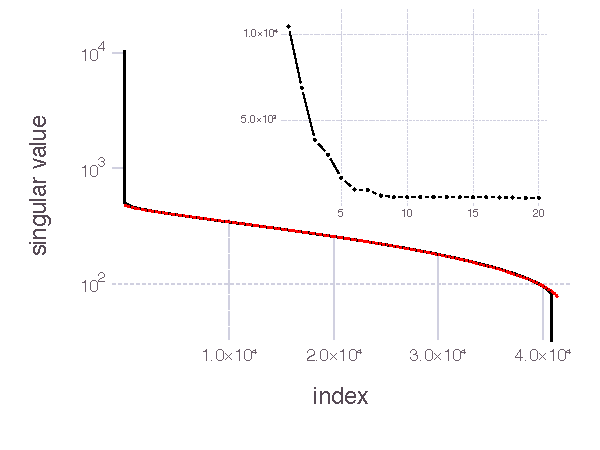
\includegraphics[width=0.45\textwidth]{fig/synthetic/fig-empirical-scree}

\caption{Left: Histogram of the singular values of a synthetic genomics data
matrix of size $41505\times81700$ (grey bars), overlaid with the Marchenko-
Pastur law for $\rho = 1.86$ (black line). Light grey vertical lines show the
presence of 18 outlying singular values whose magnitudes exceed
$1.1\sigma_+ \approx 529.7$.
Right: Scree plot of the singular values of the same matrix
(black solid lines), showing the presence of a large, low rank portion
of approximately rank 10 (inset), and an asymptotic convergence to the same
Marchenko-Pastur law (red dotted line).}
\label{fig:empirical-spectrum}
\end{figure}


The Marchenko-Pastur law describes the distribution of governs the eigenvalues
of a random covariance matrix $Y=XX^T$ formed from a data matrix $X$
of iid elements with mean 0 and finite variance $\sigma^2$.
Let $\rho$ be the ratio of the number of rows of $X$ to the number of columns of
$X$. Then, the nonzero eigenvalues follow the distribution
%
\begin{equation}
    \label{eq:mplaw-ev}
    p_e(\xi) = \frac {\sqrt{(\lambda_+-\xi)(\xi-\lambda_-)}} {2 \pi \sigma^2 \lambda x}
\end{equation}
%
where
$\lambda_+ = \sigma^2(1+\sqrt{\rho})^2$ and
$\lambda_- = \sigma^2(1-\sqrt{\rho})^2$.

When written in terms of the probability density of the singular values of $X$,
the law reads
%
\begin{equation}
    \label{eq:mplaw-sv}
    p_s(x) = \frac {\sqrt{(\sigma_+^2-x^2)(x^2-\sigma_-^2)}} {\pi \sigma^2 \min(1, \lambda) x}
\end{equation}
%
where
$\sigma_+ = \sqrt{\lambda_+} = \sigma(1+\sqrt{\rho})$ and
$\sigma_- = \sqrt{\lambda_-} = \sigma\vert1-\sqrt{\rho}\vert$.

Figure~\ref{fig:mplaw} shows typical density plots for random eigenvalues
and singular values for $\rho=1.5$.

\begin{figure}
\caption{Marchenko-Pastur law for $\rho=1.5$ (black lines) for the densities of
nonzero eigenvalues of a random covariance matrix ($XX^{T}$) and the singular
values of $X$ for iid matrix elements with mean 0 and variance 1
(black lines), corrsponding to \eqref{eq:mplaw-ev} and \eqref{eq:mplaw-sv}
respectively.
Shown for comparison are corresponding histograms (grey
bars) of numerically sampled eigenvalues and singular vectors from
a numerically sampled random matrix $X$ of size $1000\times667$,
with iid Gaussian entries of mean 0 and variance 1.
\label{fig:mplaw}
}

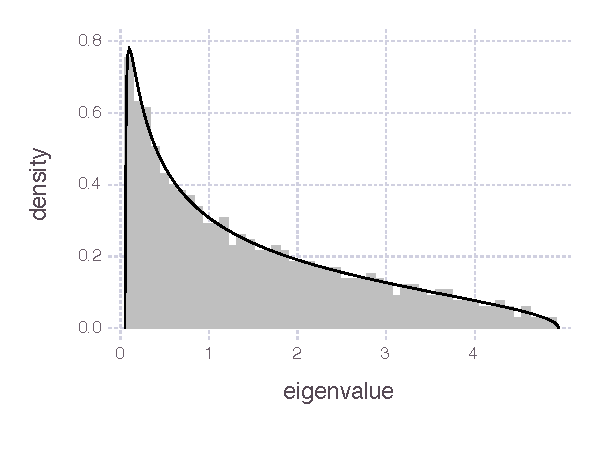
\includegraphics[width=0.45\textwidth]{fig/mplaw/fig-mplaw-ev}
%
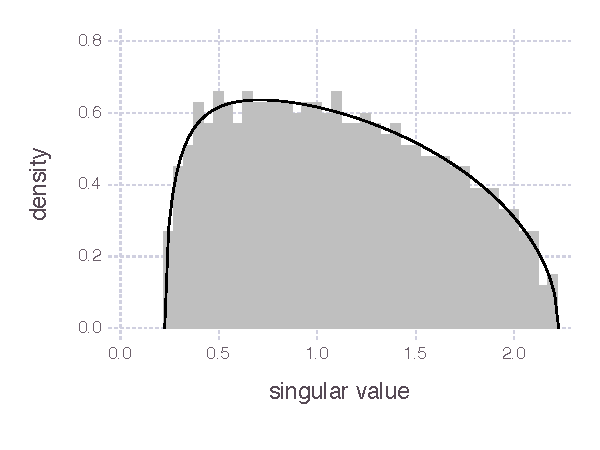
\includegraphics[width=0.45\textwidth]{fig/mplaw/fig-mplaw-sv}
\end{figure}


It is worth noting that random matrix theory had been previously introduced in
the theoretical analysis of principal components of genomics matrices.
\cite{Patterson2006} proposed a hypothesis test that computed principal components
should correspond to eigenvalues that were different from those expected from a
pure random covariance matrix,
and comparing in particular the largest eigenvalue against one randomly sampled
from the Tracy-Widom distribution~\cite{Tracy1993,Tracy1994}.
Here, we observe that the bulk distribution of singular values in genomics
matrices empirically satisfies the Marchenko-Pastur law, albeit with a
modified parameter $\rho = 1.86$ as opposed to the value $81700/41505=1.97$
which would be expected from taking the ratio of the number of rows to the
number of columns.


\section{Algorithms for PCA}

The discussion in Section~\ref{sec:model} demonstrates that the confounding
effects of population substructure can and does produce a low rank structure in
the top singular vectors, which can be captured even in the very crude random
matrix model of Algorithm~\ref{code:model}. The top few principal components,
which by construction capture the largest components of the variability, are
good candidates for modeling the unwanted variation as described in
Section~\ref{sec:regress-correction} and have been used in the statistical
genetics community for this
purpose~\cite{Chen2003,Patterson2006,Price2006,Zhu2002,Zhang2003}.

Iterative eigenvalue (or singular value)
methods~\cite{Bai2000} are therefore computationally efficient choices for
determining these principal components, as only a handful of them are needed.

The method implemented in FlashPCA~\cite{abraham2014fast} is randomized
subspace iteration one of the randomized SVD algorithms described in
\cite{halko2011finding}.

To our surprise, it does not appear that Lanczos-based bidiagonalization
methods have been used to compute principal components of genomics matrices.
We have therefore implemented Golub-Kahan-Lanczos bidiagonalization~\cite{Golub1965}
method in pure Julia. To control the memory usage and accumulation of
roundoff error, we also include an implementation of the thick restart
strategy~\cite{Stewart2001,Baglama2005} and offer the choice of full and
partial reorthogonalization~\cite{Simon1984,Larsen1998}.
Julia is a high level dynamic language for technical computing~\cite{Bezanson2012,Bezanson2015}
that provides a convenient expressive syntax close to mathematical
notation while facilitating compiler optimizations to generate fast machine
code.

\begin{algorithm}
\caption{Simple Golub-Kahan-Lanczos bidiagonalization in Julia}

\begin{lstlisting}
function svd_gkl(A, q; maxiter=minimum(size(A)))
    m, n = size(A)
    T = eltype(A)
    Tr = typeof(one(T)/norm([one(T)]))

    $α$s = Tr[]
    $β$s = Tr[]
    P = zeros(T, m, 0)
    Q = [q]

    $β$ = zero(Tr)
    p = zeros(size(A, 1))
    for iter in 1:maxiter
        p = A*q - $β$*p
	$α$ = norm(p)
        p = p/$α$
        push!($α$s, α)
        P = [P p]

        q = A'p - $α$*q
        $β$ = norm(q)
        q = q/$β$
        push!($β$s, β)
        Q = [Q q]
    end

    B = Bidiagonal($α$s, $β$s[1:maxiter-1], true)
    F = svdfact(B)
    LinAlg.SVD(P'F[:U], F[:S], F[:Vt]*Q[:,1:maxiter]')
end
\end{lstlisting}
\end{algorithm}


\subsection{Convergence analysis of FlashPCA}

Software like FlashPCA make use of randomized subspace interactions, which are
essentially equivalent to subspace iteration with a randomized starting subspace.

FlashPCA uses an unconventional convergence criterion, namely the matrix norm
of the difference between successive subspace basis vectors,
$\Vert Y_n - Y_{n-1} \Vert$.

By contrast, the standard measures of convergence using the residual norm yield
a simple error estimate for the uncertainty in a computed eigenvalues.

\cite[Theorem 4.5.1]{Parlett1998} states, in slightly altered notation, that for
any scalar $\theta$ and vector $v$, there is an eigenvalue $\lambda$ of $Y$ satisfying
\[
\vert\lambda - \theta\vert \le \Vert Y v - v \theta \Vert
\]

Notably, this result does not require that $(\theta, v)$ be a Ritz pair or have
any variational structure whatsoever. Therefore, we can use

\[
\Delta \sigma_i = \sqrt{\Vert X X^T v_i - v_i \theta_i \Vert}
\]

as an error bar for using $\sqrt{\theta_i}$ as an estimate for a singular value,
where $(\theta_i, v_i)$ is some eigenpair of $Q^T X X^T Q$ computed at any
iteration of FlashPCA.



\section{Speed and accuracy results on synthetic genomics data}

\subsection{Comparing TSVD and FlashPCA}
For our synthetic dataset the time difference between the two methods is large. The initial preprocessing steps where the matrix is read and scaled contribute very little to any of the methods. For FlashPCA, the running time consists of two major components which is an initial matrix multiply, $XX^T$, and the subsequent subspace iterations. Forming the matrix $XX^T$ is the default option in FlashPCA and might be a relict from the time when the number of gene positions (columns) was much larger the number of sample (rows). For an aspect ratio of $\frac{1}{2}$ this computation is expensive. In addition to the pure flop expense in computing $XX^T$, on our system, there is a large penalty for using Eigen relative to MKL where the former executes in 926 and the latter in 306 seconds for the same number of threads. In contrast to the algorithmic differences, this difference might be very system dependent.

The largest component of the running time for FlashPCA is the subspace iterations. By tracking the convergence criterion at each iteration it is clear that the convergence is very slow. Figure~\ref{fig:conv} shows the convergence of the FlashPCA with QR orthogonalization and our TSVD algorithm.

\begin{table}
    \caption{Running time in seconds for 41505x81700 SNP matrix}
    \centering
    \begin{tabular}{lrrr}
                                   & FlashPCA 1 & FlashPCA 2   & Julia PRO     \\
        Preprocessing              &   54        &   61        & 54            \\
        Matrix multiplication      &  971        &  926        & .             \\
        Subspace/Lanczos iteration &   41        & 1935        & 37            \\
        Postprocessing             &    7        &   11        & 0             \\
        Total                      & 1073        & 2933        & 81
    \end{tabular}
\end{table}

\begin{figure}
    \centering
    \begin{subfigure}{0.72\textwidth}
        \begin{tikzpicture}
            \begin{semilogyaxis}[width=9.5cm, height=5cm, xmin = 0, xmax = 169, ymin=10e-15, ymax=10e1]
                \addplot[very thick] file {data/FlashPCAQRconv.txt};
            \end{semilogyaxis}
        \end{tikzpicture}
        \caption{FlashPCA}
    \end{subfigure}
    \begin{subfigure}{0.23\textwidth}
        \begin{tikzpicture}
            \begin{semilogyaxis}[width=3cm, height=5cm, ymin=10e-15, ymax=10e1]
                \addplot[very thick] file {data/JuliaPCAconv.txt};
            \end{semilogyaxis}
        \end{tikzpicture}
        \caption{Julia-Lanczos}
    \end{subfigure}
    \caption{Convergence}
    \label{fig:conv}
\end{figure}


\subsection{Accuracy and speed results}

\begin{table}
\begin{tabular}{|c|c|c|c|c|c|c|c|c|}
\hline
 & Algorithm & mvps & Wall time & $\beta_{final}$ & $\left\Vert \Delta\theta\right\Vert _{1}$ & $\left\Vert \Delta\theta\right\Vert _{\infty}$\tabularnewline
\hline
\hline
FlashPCA1 & Block power & 2280 & 2616.1 sec. & 6.4 & $4\times10^{+4}$ & $4\times10^{+4}$\tabularnewline
\hline
FlashPCA2 & Block power & 2933 &  &  &  & \tabularnewline
\hline
PROPACK & GKL (PRO, NR) & 298 & 264.6 & - & $4\times10^{-8}$ & $4\times10^{-8}$\tabularnewline
\hline
ARPACK & GKL (FRO, IR) & 355 & 858.5 & 7.8 & $6\times10^{-3}$ & $1\times10^{-3}$\tabularnewline
\hline
this work & GKL (FRO, TR) & 280 & 397.8 & 6.4 & $2\times10^{-3}$ & $2\times10^{-3}$\tabularnewline
\hline
this work & GKL (PRO, NR) & 321 & 302.4 & 15072 & $6\times10^{-4}$ & $6\times10^{-4}$\tabularnewline
\hline
\end{tabular}

\caption{Comparing various methods for computing the top 20 principal
components on a simulated genotype matrix of size $41505\times81700$.
Linear algebra kernels were run on OpenBLAS v0.2.18 with 16 software threads.
FlashPCA1 - Reimplementation in pure Julia of the published version of FlashPCA,
FlashPCA2 - Reimplementation in pure Julia of the master version of FlashPCA available on GitHub,
GKL - Golub--Kahan--Lanczos bidiagonalization,
PRO - partial reorthogonalization,
FRO - full reorthogonalization,
NR - no restart,
IR - implicit restart after 40 Lanczos vectors,
TR - thick restart after 40 Lanczos vectors,
mvps - number of matrix--vector products.
Termination criterion set to $\Vert Y\Vert = 10^{-8}$ for FlashPCA$n$,
and relative error in the singular values of $10^{-8}$ for the Lanczos methods.
}
\end{table}

\begin{figure}
\caption{Convergence behavior of Lanczos with partial reorthogonalization. Top 20 singular values requested.}
\label{fig:conv-lanczos-tsvd}
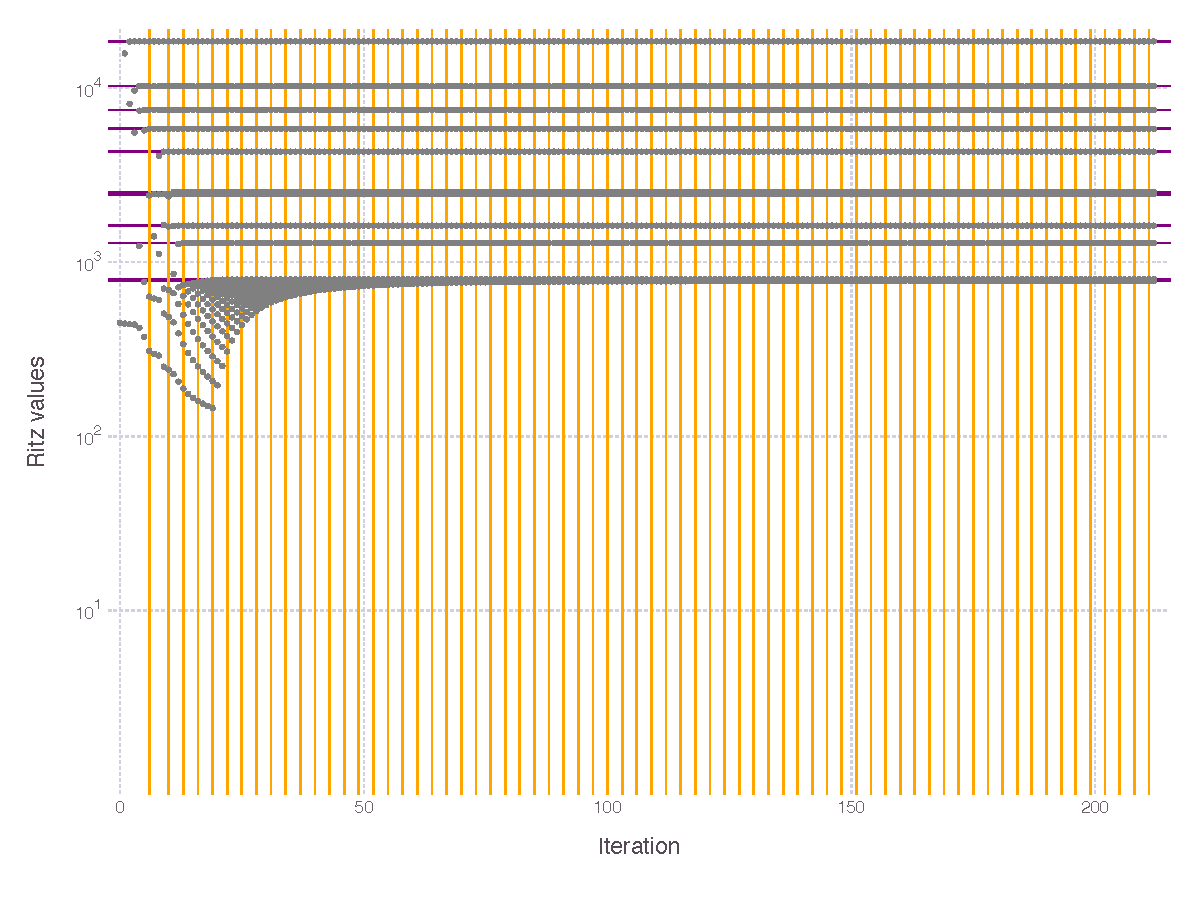
\includegraphics[width=\textwidth]{fig/tsvdconv}
\end{figure}

\begin{figure}
\caption{Errors of Ritz values for Lanczos with partial reorthogonalization. Top 20 singular values requested.}
\label{fig:error-lanczos-tsvd}
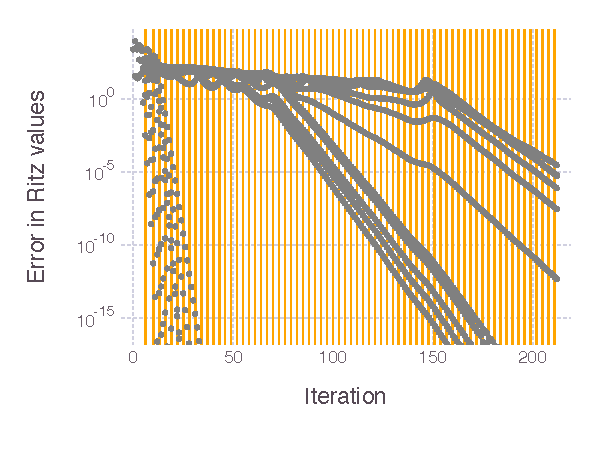
\includegraphics[width=\textwidth]{fig/tsvderror}
\end{figure}

\begin{figure}
\caption{Convergence behavior of thick-restarted Lanczos with full reorthogonalization, with top 20 singular values requested. Restarts were triggered every 40 microiterations (grey vertical lines).
\label{fig:lanczos-tr}
}

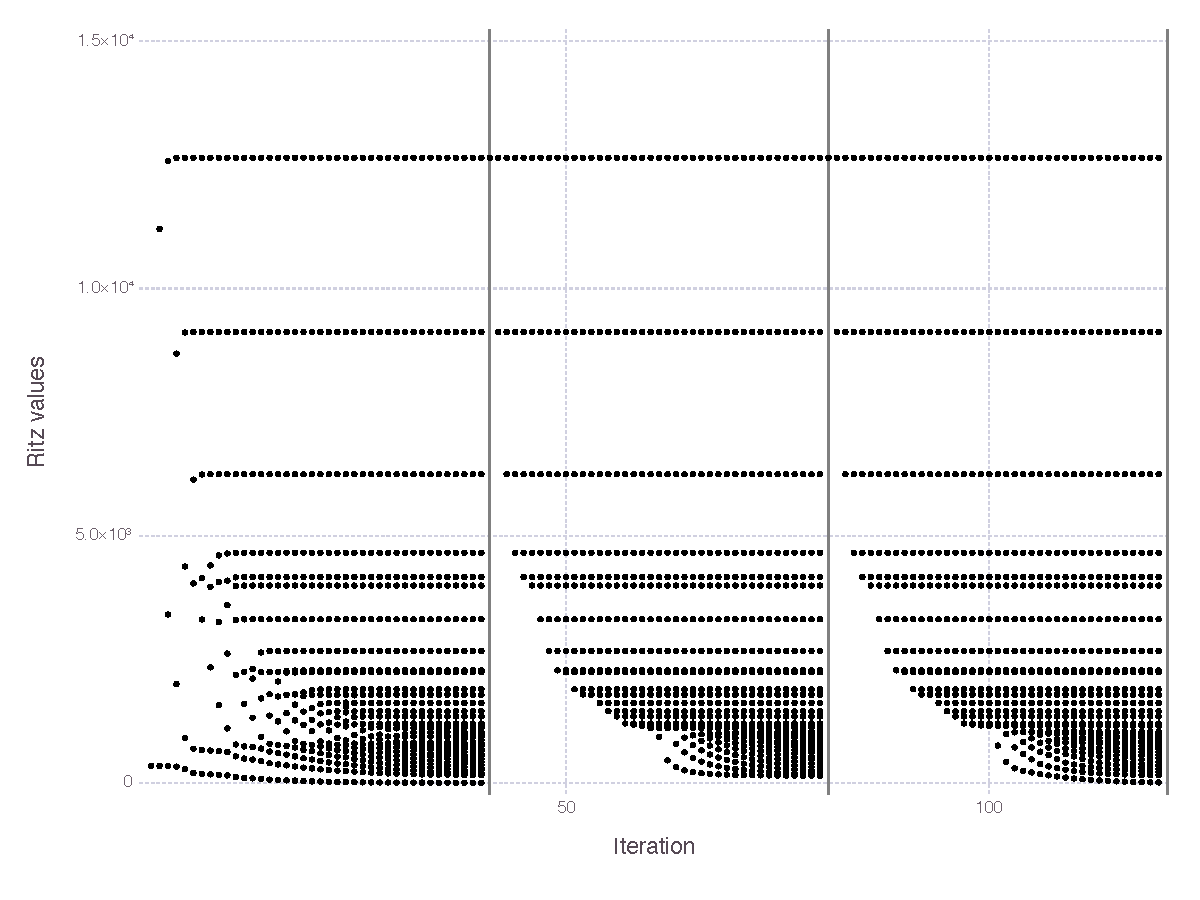
\includegraphics[width=\textwidth]{fig/thickrestarted/fig-conv}
\end{figure}

\begin{figure}
    \centering
    \begin{tikzpicture}
        \begin{semilogyaxis}[width=10cm, height=5cm]
            \addplot[very thick, mark=*] file {data/condNumberNorm.txt};
        \end{semilogyaxis}
    \end{tikzpicture}
    \caption{Condition number of the matrix of subspace basis per iteration for FlashPCA without QR. The condition number at iteration zero is the condition number of the normalized basis after the initial range computation.}
\end{figure}

\section{Conclusions}

The classic Lanczos bidiagonalization methods provide a numerically efficient
method for quickly computing the largest few principal components of genomics
data matrices. The implementation of these methods in the Julia programming
language provides a fast, practical software tool that allows for easy
introspection into the inner workings of the Lanczos algorithms.

Further work remains to be done to provide the ability to do both partial
reorthogonalization and thick restart in Julia, as well well as providing
block Lanczos.

\section*{Acknowledgments}

We thank the Julia development community for their contributions to free and
open source software. Julia is free software that can be downloaded from
\url{julialang.org/downloads}. The implementation of iterative SVD described in
this paper is available as the \verb|svdl| function in the
\href{https://github.com/JuliaLang/IterativeSolvers.jl}{IterativeSolvers.jl}
package. J.C. would also like to thank Jack Poulson (Stanford) and David Silvester
(Manchester) for many insightful discussions.

\bibliography{bio,svd}

\end{document}
